\documentclass[12pt]{beamer}
\usetheme{LMT}
\usepackage[utf8]{inputenc}
\usepackage{multido}
\usepackage{calc}
\usepackage{ifthen}
\usepackage[absolute,overlay]{textpos} %[showboxes,absolute,overlay]{textpos}

%\setlength{\TPHorizModule}{\paperwidth}\setlength{\TPVertModule}{\paperheight}
\setlength{\TPHorizModule}{1cm} % échelle horizontale
\setlength{\TPVertModule}{\TPHorizModule} % échelle verticale identique à l'horizontale

\title[PGD - Dynamics]{PGD for low frequency dynamics problems involving localized non-linearities}
%\subtitle{}
\author{ \textsc{P. Nargil} \\  \textsc{F. Louf} and \textsc{P.A. Boucard}}
\institute{LMT Cachan}
\date{Friday 5th December 2014}

\newcommand\Fontvi{\fontsize{6}{7.2}\selectfont}
\newcommand\Fontplan{\fontsize{9.5}{11}\selectfont}
\newcommand\FontGoal{\fontsize{9.5}{11}\selectfont}
\newcommand\FontMethod{\fontsize{10}{12}\selectfont}
\newcommand\FontPOD{\fontsize{10}{12}\selectfont}
\newcommand\FontPersp{\fontsize{10}{12}\selectfont}
\newcommand\FontBiblio{\fontsize{8.5}{10}\selectfont}
\newcommand\FontBiblioT{\fontsize{9.5}{11}\selectfont}


\graphicspath{{figures/}}
% ---------------------------------------------------------------------
\begin{document}
\frame{\titlepage}
\author{ \textsc{P. Nargil}}
% ---------------------------------------------------------------------
%\frame{\tableofcontents}
%\addtocounter{framenumber}{3}


\section{MECASIF Project}

\begin{frame}{
\includegraphics[width=1\linewidth ,height=1.5cm,keepaspectratio]{Logo/MECASIF.pdf}} 
\newcommand\N{6}
	\multido{\iX=1+1,\iY=1+\N}{6}{%
		\begin{figure}
	  		\multido{\iZ=\iY+1,\iA=1+1}{\N}{%
			\begin{minipage}{0.14\linewidth}
			\ifthenelse{\iX=1}
				{\centering \includegraphics[width=1\linewidth ,height=1cm,keepaspectratio]{Logo/Z\iZ.png}}
				{
					\ifthenelse{\iA=1}
					{\centering \includegraphics[width=1\linewidth ,height=1cm,keepaspectratio]{Logo/Z\iZ.png}}
					{
						\ifthenelse{\iA=\N}
						{\centering \includegraphics[width=1\linewidth ,height=1cm,keepaspectratio]{Logo/Z\iZ.png}}
						{\hspace{1\linewidth}}
					}
				}
			%\centering \includegraphics[width=1\linewidth ,height=1.5cm,keepaspectratio]{Logo/Z\iZ.png}
			\end{minipage}
			}
		\end{figure}
		\vspace{-0.2cm}
	}
	\begin{textblock}{6}[0,0](4,3.5)
	Main Subprojects
		\begin{itemize}
			\item Project Leading %Gouvernance du project
			\item Transversal Methods %Méthodes transverses
			\item \underline{Non Linear Vibrations} %Vibration non linéaire
			\item Fast Dynamics %Dynamique rapide
			\item Fluid Dynamics %Dynamique des fluides
			\item Promoting \& Broadcasting %Promotion & Dissémination
		\end{itemize}
	\end{textblock}
\end{frame}

\begin{frame}{
\includegraphics[width=1\linewidth ,height=1.5cm,keepaspectratio]{Logo/MECASIF.pdf}} 
\newcommand\N{6}
	\multido{\iX=1+1,\iY=1+\N}{6}{%
		\begin{figure}
	  		\multido{\iZ=\iY+1,\iA=1+1}{\N}{%
			\begin{minipage}{0.14\linewidth}
			\centering 
			\ifthenelse{\iX=1}
				{\includegraphics[width=1\linewidth ,height=1cm,keepaspectratio]{LogoT/Z\iZ.png}}
				{
					\ifthenelse{\iA=1}
					{\includegraphics[width=1\linewidth ,height=1cm,keepaspectratio]{LogoT/Z\iZ.png}}
					{
						\ifthenelse{\iA=\N}
						{\includegraphics[width=1\linewidth ,height=1cm,keepaspectratio]{LogoT/Z\iZ.png}}
						{\hspace{1\linewidth}}
					}
				}
			%\centering \includegraphics[width=1\linewidth ,height=1.5cm,keepaspectratio]{Logo/Z\iZ.png}
			\end{minipage}
			}
		\end{figure}
		\vspace{-0.2cm}
	}
	\begin{textblock}{6}[0,0](4,4.5)
		\begin{itemize}
			\item Non Linear Vibrations
			\\work packages :
				\begin{itemize}
					\item Stakes and Goals
					\item Use cases 
					\item Non-Intrusive  Methods 
					\item \underline{Intrusive Methods}
				\end{itemize}
		\end{itemize}
	\end{textblock}
\end{frame}

\begin{frame}{Non Linear Vibrations - Use case}
	\vspace{-0.4cm}
	\begin{center}
		\begin{figure}
		\begin{minipage}{0.70\linewidth}
				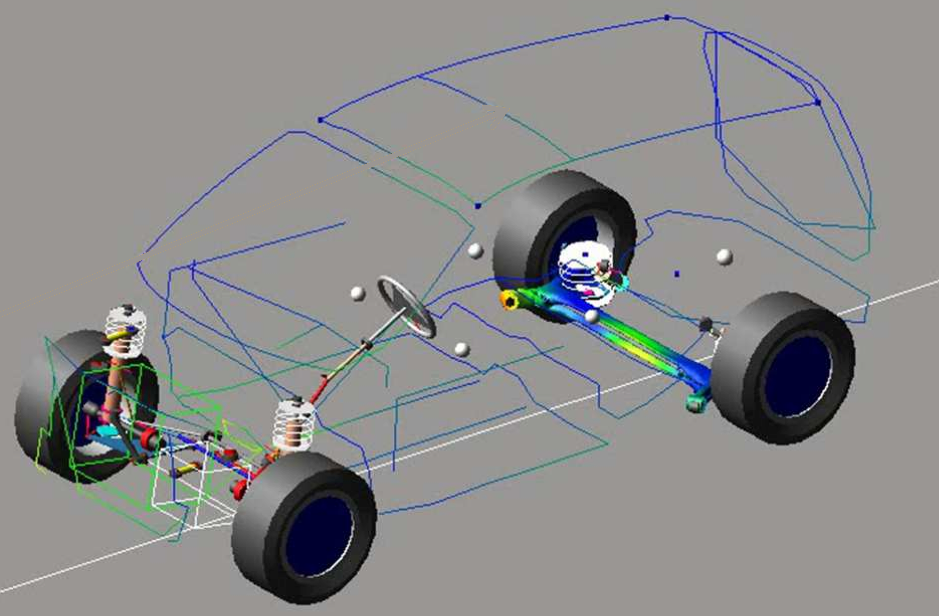
\includegraphics[width=1\linewidth]{roulage2.png}
			\end{minipage}
		\end{figure}
	\end{center}
	\vspace{-0.3cm}
	\begin{itemize}
		\item Calculation time
		\item Set of parameters
		\item Non-linearity
	\end{itemize}
\end{frame}

\begin{frame}{Presentation plan}
	\Fontplan
	\begin{block}{}
		%\vfill
			\hspace{1cm}
			\begin{minipage}[l][0.650\textheight]{0.50\linewidth}
				\setcounter{tocdepth}{2}
				\tableofcontents
			\end{minipage}
			\vspace{0.5cm}
	\end{block}
\end{frame}


\section{Model Order Reduction}

\begin{frame}{Model order reduction}
\FontGoal
	Reducing calculation time by reducing the dimension of the problem
	\begin{block}{Stakes of time saving}
	{
	\begin{itemize}
	\item Reducing the developement cost
	\item Optimisation / Creation of probabilistic models
	\item Solving of problems reaching calculating machine's limits
	\end{itemize}
	}
	\end{block}
	
	Reduced order modeling : Solving projected problems\\
	How to obtain the basis to project on :
	\begin{block}{Reduction methods}
	{
	\begin{itemize}
	\item POD - Proper Orthogonal Decomposition [A. Chatterjee - 2000]
	\item PGD - Proper Generalized Decomposition [P. Ladevèze - 1989]
	\end{itemize}
	}
	\end{block}
	
	% La réduction de modèles apporte une réduction du temps de calcul. 
	% En réduisant la dimension du problème, 
	%	on diminue le nombre d'opérations nécessaires à sa résolution.
	%
	% La réduction de modèles consiste à résoudre un problème 
	%	après l'avoir projeté sur une base de dimension inférieure
	%	à celle de la base d'origine.
	% Il existe différentes méthodes pour obtenir ces bases.

\end{frame}

\begin{frame}%{Bibliography}
Construction of the Reduced-Order Basis, bibliography

\FontBiblioT
\begin{itemize} \leftmargini5pt \leftmarginii2pt \leftmarginiii0pt
	\item offline/online techniques
		\begin{itemize}
			\FontBiblio
			\item Proper Orthogonal Decomposition (POD) %\hspace{-1cm} \hfill \\
				\begin{itemize}% \itemsep1pt \parskip0pt \parsep0pt
					\FontBiblio
					\item[] [Sirovich~87] [Holmes~et~al.~93] [Krysl~et~al.~00] [Kunisch,Wolkwein~02]
					[Willcox~et~al.~02] [Picinbono~et~al.~03] [Bergmann~et~al.~05] [Lieu~et~al.~06] 
					[Gunzburger~et~al.~06] [Niroomandi~et~al.~08] [Farhat~et~al.~08] [Matthies~et~al.~10]~...
					also known as KLD [Karhunen~43] [Loeve~55], PCA [Pearson~1901], [Hotteling~33]. 
					In finite dimension SVD [Ekardt~\&~Young39], and if more than 2 variables HOSVD [Baranyi~et~al.06]		
				\end{itemize}
			\item Reduced-Basis (RB)
				\begin{itemize}
					\FontBiblio
					\item[] [Maday~et~al.~02] [Patera~et~al.~02] [Rozza~et~al.~07] [Haasdonk~et~al.~08] [Boyaval~et~al.~09] ...				
				\end{itemize}			
		\end{itemize}
		\vspace{-0.2cm}
					\FontBiblioT
		\item On-the-fly techniques - PGD - review article [Chinesta,~Ladevèze,~Cueto11]
					\FontBiblio
			\begin{itemize}
					\FontBiblio
				\item Radial approximation (PGD time/space)
				\begin{itemize}
					\FontBiblio
					\item[] [Ladevèze 85, 99] ... [Ladevèze et al. 99-11] [Nouy et Ladevèze 03, 04] [Ladevèze, Dureissex, Néron 04]
					[Ladevèze et al. 08, 09, 10] [Néron and Dureisseix 08] [Boucard and Néron 11, 12] ...
				\end{itemize}	
					\item Generalized spectral decomposition
						\begin{itemize}
						\FontBiblio
						\item[]  [Nouy et al. 07-12]
						\end{itemize}
					\FontBiblio
					\item Multidimensional separation - PGD time/space/parameter
						\begin{itemize}
						\FontBiblio
						\item[] [Ammar~and~Chinesta~06] [Ryckelynck~06] [Chinesta~et~al.~08-11] [Beringhier~et~al.~10]~...
						\end{itemize}						

			\end{itemize}
\end{itemize}

\end{frame}

%\begin{frame}{Bibliography}
%Construction of the Reduced-Order Basis
%
%\begin{itemize}
%	\item offline/online techniques
%		\begin{itemize}
%			\FontBiblio
%			\item Proper Orthogonal Decomposition (POD)
%				\begin{itemize}
%					\FontBiblio
%					\item[] [Sirovich~87] [Holmes~et~al.~93] [Krysl~et~al.~00] [Kunisch,Wolkwein~02]
%					[Willcox~et~al.~02] [Picinbono~et~al.~03] [Bergmann~et~al.~05] [Lieu~et~al.~06] 
%					[Gunzburger~et~al.~06] [Niroomandi~et~al.~08] [Farhat~et~al.~08] [Matthies~et~al.~10]~...				
%				\end{itemize}
%			\item Reduced-Basis (RB)
%				\begin{itemize}
%					\FontBiblio
%					\item[] [Maday~et~al.~02] [Patera~et~al.~02] [Rozza~et~al.~07] [Haasdonk~et~al.~08] [Boyaval~et~al.~09] ...				
%				\end{itemize}			
%		\end{itemize}
%		\item On-the-fly techniques
%			\begin{itemize}
%				\item Proper Generalized Decomposition (PGD)
%				\begin{itemize}
%					\FontBiblio
%					\item[] [Ladevèze~85,~99] ... [Ladevèze~et~al.~99-14] [Allix~et~al.~02] [Néron,~Ladevèze~03-14] [Néron,~Dureisseix~08] [Néron,~Boucard,~11-14] [Nouy~et~al.~07-14] [Chinesta, Ammar, Cueto, Huerta, Diez, Gonzalez, Leygue, Bordeu...~06-14] [Ryckelynck~05-] [Joyot~et~al.~08-] [Beringhier~et~al.~10-] [Hamdouni~et~al.~11]~...
%					\item[] [Falco~et~al.~07-] [Maday~et~al.~09-] [Lelièvre~et~al.~11-]~...	
%				\end{itemize}	
%			\end{itemize}
%\end{itemize}
%
%\end{frame}

\section{Different methods}

\begin{frame}{Presentation plan}
\Fontplan
\addtocounter{framenumber}{-1}
	\begin{block}{}
		%\vfill
			\hspace{1cm}
			\begin{minipage}[l][0.650\textheight]{0.50\linewidth}
				\setcounter{tocdepth}{2}
				\tableofcontents[currentsection] 
			\end{minipage}
			\vspace{0.5cm}
	\end{block}
\end{frame}


\begin{frame}{Different methods}
\FontMethod
	\begin{figure}
   \begin{minipage}{0.47\linewidth}
		\begin{alertblock}{POD}
		\vbox to .7\textheight{%
			\begin{itemize}
			\item a posteriori or \\ offline/online technique
			\item give modes in:
				\begin{itemize}
				\item space
				\item time
				\end{itemize}
			\end{itemize}
			\vspace{0.55cm}
			\begin{itemize}
			\item Principle :
			\end{itemize}
			Projection on a basis of modes exctracted from truncated SVD
			%	À partir de la solution d'un problème à laquelle 
			%	on applique une SVD, on trouve les modes principaux 
			%	associés aux valeurs singulières les plus élevées.
			\vfill
		}
		\end{alertblock}
   \end{minipage}\hfill
   \begin{minipage}{0.47\linewidth}
		\begin{exampleblock}{PGD}
		\vbox to .7\textheight{%
			\begin{itemize}
			\item modes calculation on the fly
			\vspace{0.45cm}
				\item give modes in :
					\begin{itemize}
					\item space
					\item time
					\item parameter
					\end{itemize}
			\end{itemize}
			\begin{itemize}
			\item Principle :
			\end{itemize}
			Modes calculated using an iterative method (fixed point)
			 at the same time as the resolution.	
			%	À partir des données d'un problème on calcule les modes 
			%	"à la volée" par une méthode de point fixe en résolvant.
			\vfill
		}
		\end{exampleblock}
   \end{minipage}
\end{figure}

\end{frame}


\subsection{POD}

\begin{frame}{Proper Orthogonal Decomposition}
	\FontPOD
	\begin{alertblock}{A dynamic problem is solved on the system, and the SVD gives :}
	$ \displaystyle U(X,t) = \sum_{k=1}^{dim} V_{Sk}~f_k(X) g_k(t)$\\
	\end{alertblock}
		
	\begin{alertblock}{The basis is obtained by truncating the result}
	The $n$ modes $f_k(X)$ associated to the highest 
	singular values are chosen to make the reduced basis.\\
	The SVD guarantees the best truncated basis such as :
	$ \displaystyle U(X,t) - U_n(X,t) = U(X,t) - \sum_{k=1}^{n} V_{Sk}~ f_k(X) g_k(t)$\\
	is minimal for a fixed $n$ (in Frobenius norm).\\
	These couples are the most representative ones of the studied response.
	\end{alertblock}
	\vspace{-0.3cm}
	\begin{figure}
	$~$
	   \begin{minipage}{0.19\linewidth}
			\begin{alertblock}{}
				\centering		
				Solving (Snapshot)
				%\vspace{0.22cm}
			\end{alertblock}
	   \end{minipage}\hfill
	   \begin{minipage}{0.03\linewidth}
			\vspace{0.220cm}
	   		$\!\!\rightarrow$
	   \end{minipage}\hfill
	   \begin{minipage}{0.19\linewidth}
			\begin{alertblock}{}
				\centering		
				%\vspace{0.210cm}
				Getting the reduced basis
				%\vspace{0.22cm}
			\end{alertblock}
	   \end{minipage}
	   \begin{minipage}{0.03\linewidth}
			\vspace{0.220cm}
	   		$\!\!\!\rightarrow$
	   \end{minipage}\hfill
	   \begin{minipage}{0.19\linewidth}
			\begin{alertblock}{}
				\centering		
				Projection on the RB
			\end{alertblock}
	   \end{minipage}\hfill
	   \begin{minipage}{0.03\linewidth}
			\vspace{0.220cm}
	   		$\!\!\rightarrow$
	   \end{minipage}\hfill
	   \begin{minipage}{0.19\linewidth}
			\begin{alertblock}{}
				\centering		
				\vspace{0.20cm}
				Solving
				\vspace{0.20cm}
			\end{alertblock}
	   \end{minipage}
	\end{figure}
		
\end{frame}

\subsection{PGD}

\begin{frame}{Proper Generalized Decomposition}
	\FontPOD
	\begin{exampleblock}{Approximation using separable variables}
	$ \displaystyle U_n(X,t,\lambda) = \sum_{k=1}^n 
											f_k(X) g_k(t) h_k(\lambda)$
	\end{exampleblock}
	\vspace{-0.1cm}
	\begin{exampleblock}{The variational formulation gives a problem for each type of function}
	$ f_k = F (U_{k-1},g_k,h_k)~,~~~~~
	 g_k = G (U_{k-1},f_k,h_k)~,~~~~~
	 h_k = H (U_{k-1},f_k,g_k)$
	\end{exampleblock}
	\vspace{-0.4cm}
	\begin{figure}[t]
	$~$
	   \begin{minipage}[l]{0.40\linewidth}
			\begin{exampleblock}{Algorithm}
			\vbox to .4\textheight{%
				\vspace{0.42cm}
				$ ~~for~k = 1$ à $ n$ \\
				$ ~~\phantom{for} for~j=1$ à $j_{max}$ \\
				$ ~~\phantom{for for~j } f_k = F (U_{k-1},g_k,h_k)$ \\
				$ ~~\phantom{for for~j } g_k = G (U_{k-1},f_k,h_k)$ \\
				$ ~~\phantom{for for~j } h_k = H (U_{k-1},f_k,g_k)$ \\
				$ ~~\phantom{for} end$ \\
				$ ~~end $ \\				
			}
			\end{exampleblock}
	   \end{minipage}\hspace{0.05cm}
	   \begin{minipage}{0.52\linewidth}
			\begin{exampleblock}{Details \phantom{g}}
			\vbox to .4\textheight{%
				\[
				\begin{array}{l}
				~\text{Iterating on the modes }\\
				~ \phantom{for}\text{Using a fixed point loop}\\
				\phantom{for for}
				~\left\{
				\begin{array}{l l}
				&\!\!\!\!\!\!\!\!f_k = F (U_{k-1},g_k,h_k) \\
				&\!\!\!\!\!\!\!\!g_k = G (U_{k-1},f_k,h_k) \\
				&\!\!\!\!\!\!\!\!h_k = H (U_{k-1},f_k,g_k) \\				
				\end{array}
				\right.			\\
				~ \phantom{for}\text{to solve the non-linear problem.} \\
				~\text{until you reach }n\text{ modes.}\\			
				\end{array}
				\]
			}
			\end{exampleblock}
	   \end{minipage}
	\end{figure}
	
\end{frame}


\section{A few results}

\begin{frame}{Presentation plan}
\Fontplan
\addtocounter{framenumber}{-1}
	\begin{block}{}
		%\vfill
			\hspace{1cm}
			\begin{minipage}[l][0.650\textheight]{0.50\linewidth}
				\setcounter{tocdepth}{2}
				\tableofcontents[currentsection] 
			\end{minipage}
			\vspace{0.5cm}
	\end{block}
\end{frame}



\subsection{Error}

\begin{frame}{Error indicators}
%	\begin{equation}
%		e_ {Amp} = \left|\frac{max(s_ {Ref}) - min(s_ {Ref}) 
%							- \big[ max(s_ {Cal}) - min(s_ {Cal}) \big] }
%		{max(s_ {Ref}) - min(s_ {Ref})} \right|
%	\end{equation}

%	\begin{equation}
%		e_ {Max} = \left|\frac{ max(s_ {Ref} - s_ {Cal}) }
%		{max(s_ {Ref}) - min(s_ {Ref})} \right|
%	\end{equation}

\begin{figure}
	\begin{minipage}{0.45\linewidth}
			
\includegraphics[width=1\linewidth]{Beam-tikz-0.eps}
			\caption{\centering Academical problem}		
	\end{minipage}
	\end{figure}
		
	 Relative error (obtained with reference solution) :
	\begin{figure}
		\begin{minipage}{0.45\linewidth}
			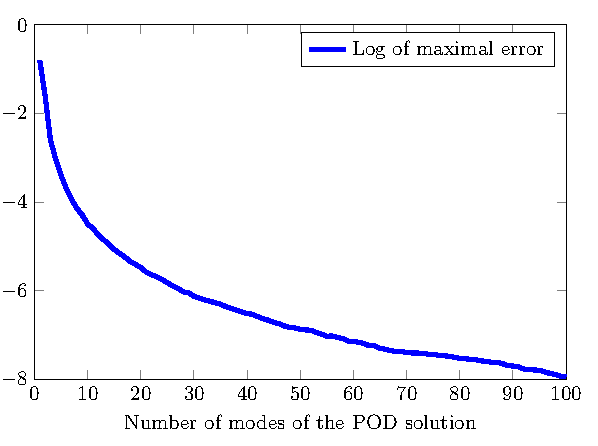
\includegraphics[width=1\linewidth]{Calcul100MPOD.eps}
			\caption{\centering POD Solution}		%{\centering Evolution of error indicators for a POD Solution}		
		\end{minipage}
		 \hspace{0.5cm}
		\begin{minipage}{0.45\linewidth}
			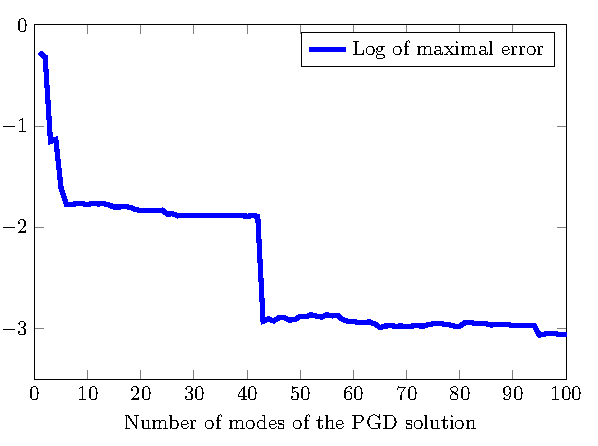
\includegraphics[width=1\linewidth]{Calcul100MPGD.eps}
			\caption{\centering PGD Solution}		
		\end{minipage}
	\end{figure}
	
\end{frame}


%\subsection{Loading velocity}
%
%\begin{frame}{Different Loading Velocities} 
%	Loading in Sinus Verse for different period lengths :
%	
%	\begin{figure}
%		\begin{minipage}[b]{0.4\linewidth}
%			
\includegraphics[width=1\linewidth]{Beam-tikz.eps}
%		\end{minipage}
%		 \hspace{1cm}
%		\begin{minipage}[b]{0.4\linewidth}
%			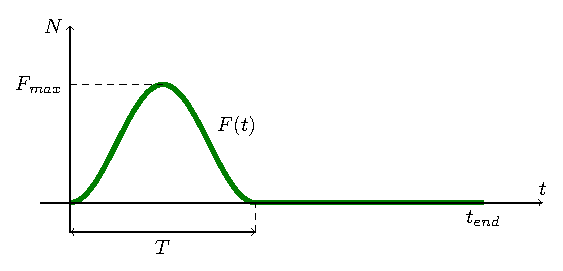
\includegraphics[width=1\linewidth]{SinVerse-tikz.eps}
%		\end{minipage}
%	\end{figure}
%	%Chargement en sinus verse pour différentes rapidités : 
%	\begin{figure}
%		\begin{minipage}{0.24\linewidth}
%			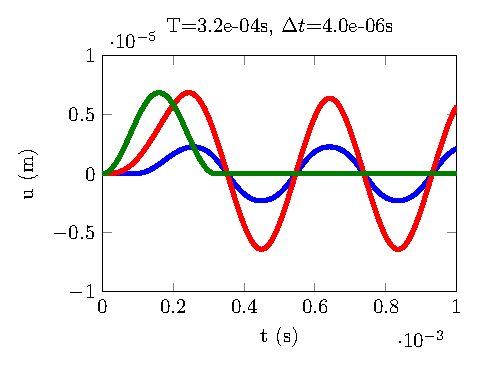
\includegraphics[width=1\linewidth]{CalculSchem3-T4-tikz.eps}
%		\end{minipage}
%		\begin{minipage}{0.24\linewidth}
%			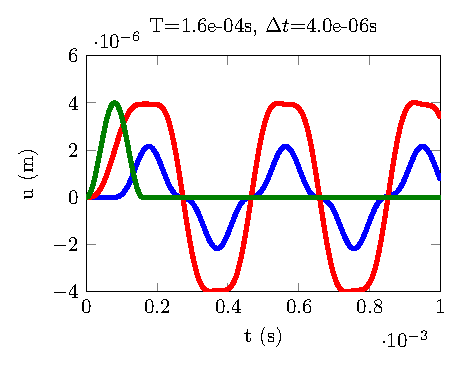
\includegraphics[width=1\linewidth]{CalculSchem3-T3-tikz.eps}
%		\end{minipage}
%		\begin{minipage}{0.24\linewidth}
%			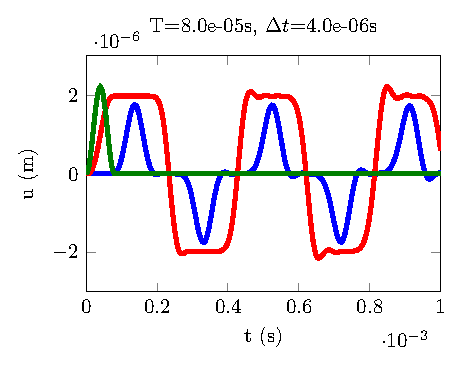
\includegraphics[width=1\linewidth]{CalculSchem3-T2-tikz.eps}
%		\end{minipage}
%		\begin{minipage}{0.24\linewidth}
%			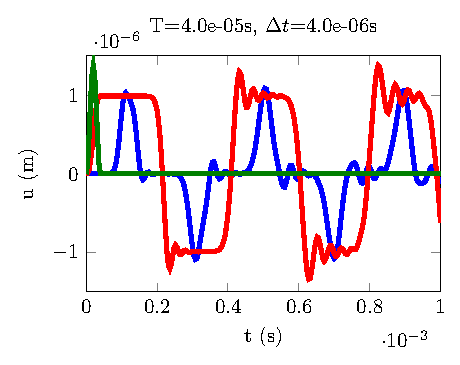
\includegraphics[width=1\linewidth]{CalculSchem3-T1-tikz.eps}
%		\end{minipage}
%	\end{figure}
%	\vspace{-0.4cm}
%	
%	\begin{figure}
%		\begin{minipage}{0.24\linewidth}
%			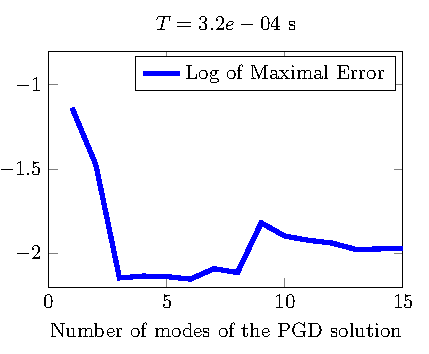
\includegraphics[width=1\linewidth]{Error-CalculSchem3-T4-tikz.eps}
%		\end{minipage}
%		\begin{minipage}{0.24\linewidth}
%			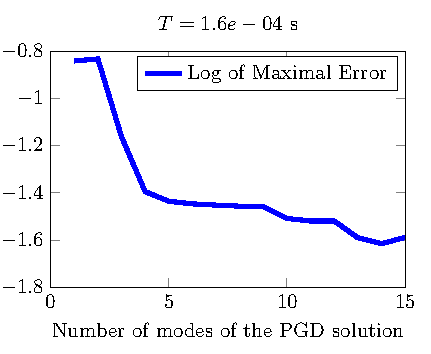
\includegraphics[width=1\linewidth]{Error-CalculSchem3-T3-tikz.eps}
%		\end{minipage}
%		\begin{minipage}{0.24\linewidth}
%			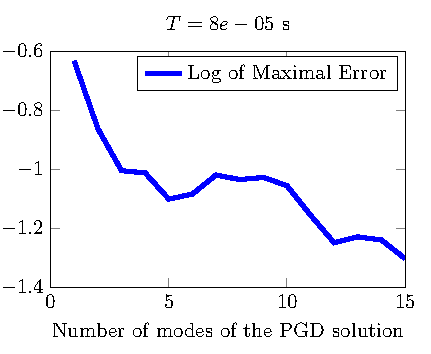
\includegraphics[width=1\linewidth]{Error-CalculSchem3-T2-tikz.eps}
%		\end{minipage}
%		\begin{minipage}{0.24\linewidth}
%			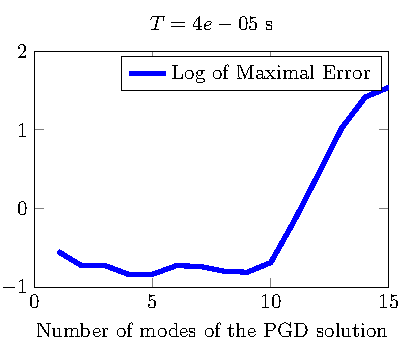
\includegraphics[width=1\linewidth]{Error-CalculSchem3-T1-tikz.eps}
%		\end{minipage}
%	\end{figure}
%\end{frame}
%
%\begin{frame}{Different Loading Velocities} 
%	\begin{figure}
%		\begin{minipage}{0.24\linewidth}
%			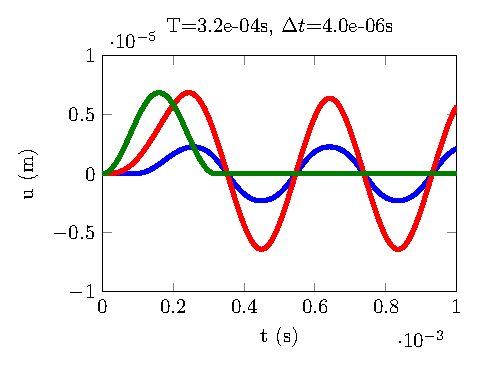
\includegraphics[width=1\linewidth]{CalculSchem3-T4-tikz.eps}
%		\end{minipage}
%		\begin{minipage}{0.24\linewidth}
%			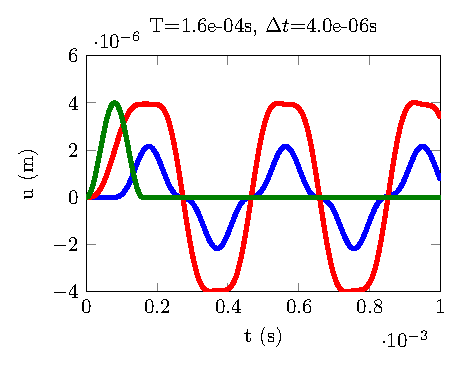
\includegraphics[width=1\linewidth]{CalculSchem3-T3-tikz.eps}
%		\end{minipage}
%		\begin{minipage}{0.24\linewidth}
%			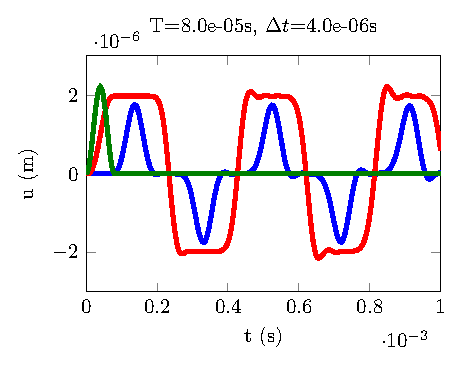
\includegraphics[width=1\linewidth]{CalculSchem3-T2-tikz.eps}
%		\end{minipage}
%		\begin{minipage}{0.24\linewidth}
%			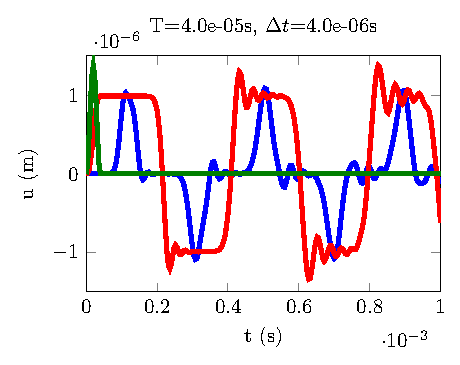
\includegraphics[width=1\linewidth]{CalculSchem3-T1-tikz.eps}
%		\end{minipage}
%	\end{figure}
%	\vspace{-0.6cm}
%	\begin{itemize}
%		\item Getting closer to a choc problem : presence of waves
%			\vspace{-0.2cm}
%		\item Presence of numerical perturbations of high frequencies
%	\end{itemize}
%	\vspace{-0.5cm}
%	
%	\begin{figure}
%		\begin{minipage}{0.24\linewidth}
%			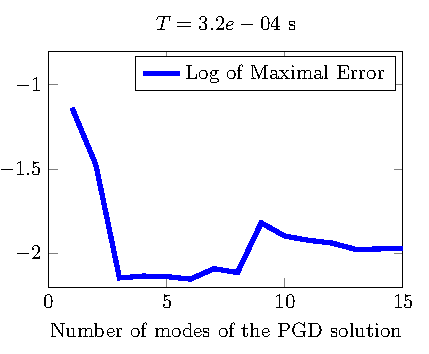
\includegraphics[width=1\linewidth]{Error-CalculSchem3-T4-tikz.eps}
%		\end{minipage}
%		\begin{minipage}{0.24\linewidth}
%			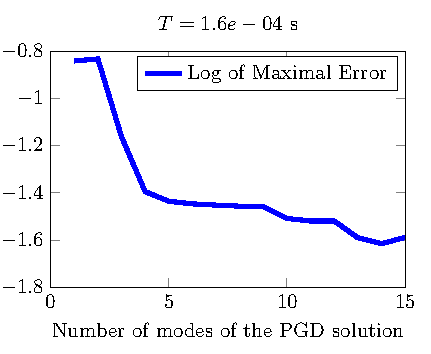
\includegraphics[width=1\linewidth]{Error-CalculSchem3-T3-tikz.eps}
%		\end{minipage}
%		\begin{minipage}{0.24\linewidth}
%			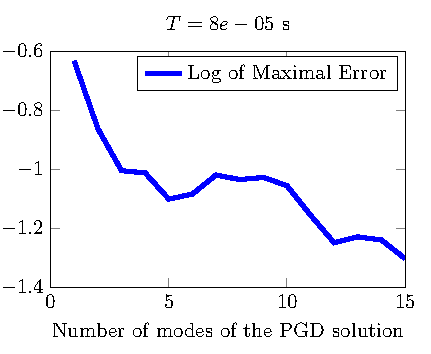
\includegraphics[width=1\linewidth]{Error-CalculSchem3-T2-tikz.eps}
%		\end{minipage}
%		\begin{minipage}{0.24\linewidth}
%			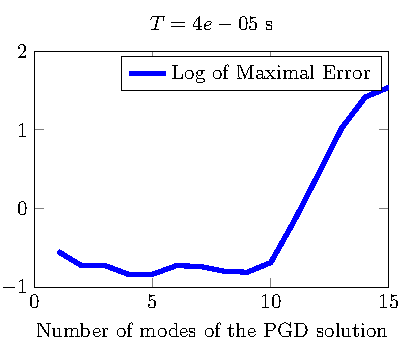
\includegraphics[width=1\linewidth]{Error-CalculSchem3-T1-tikz.eps}
%		\end{minipage}
%	\end{figure}
%	\vspace{-0.5cm}
%	\begin{itemize}
%		\item Convergence depending on loading velocity / frequency
%	\end{itemize}
%\end{frame}
%

\subsection{MAC}

\begin{frame}{MAC Analysis 
	$\frac{\left(\boldsymbol{\varphi_i.\psi_j}\right)^2}{\boldsymbol{\varphi_i.\varphi_i \times \psi_j.\psi_j}}$} 
	\begin{figure}
		\begin{minipage}{0.46\linewidth}
			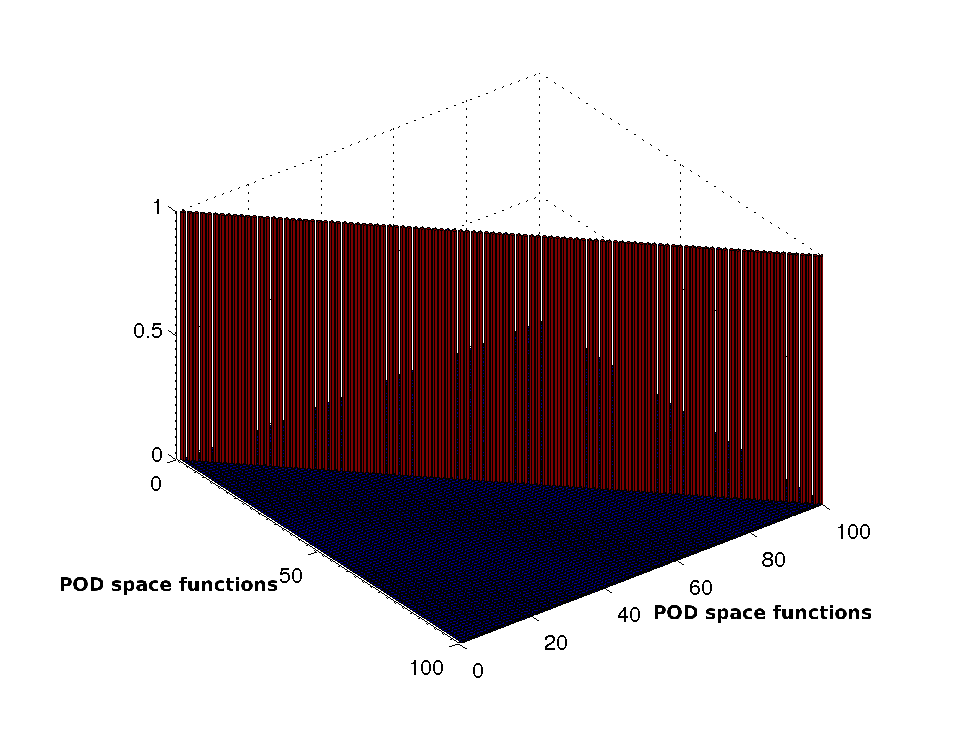
\includegraphics[width=1\linewidth]{MAC-POD2.eps}
			\caption{\centering POD space functions}		
		\end{minipage}
		 \hspace{0.5cm}
		\begin{minipage}{0.46\linewidth}
			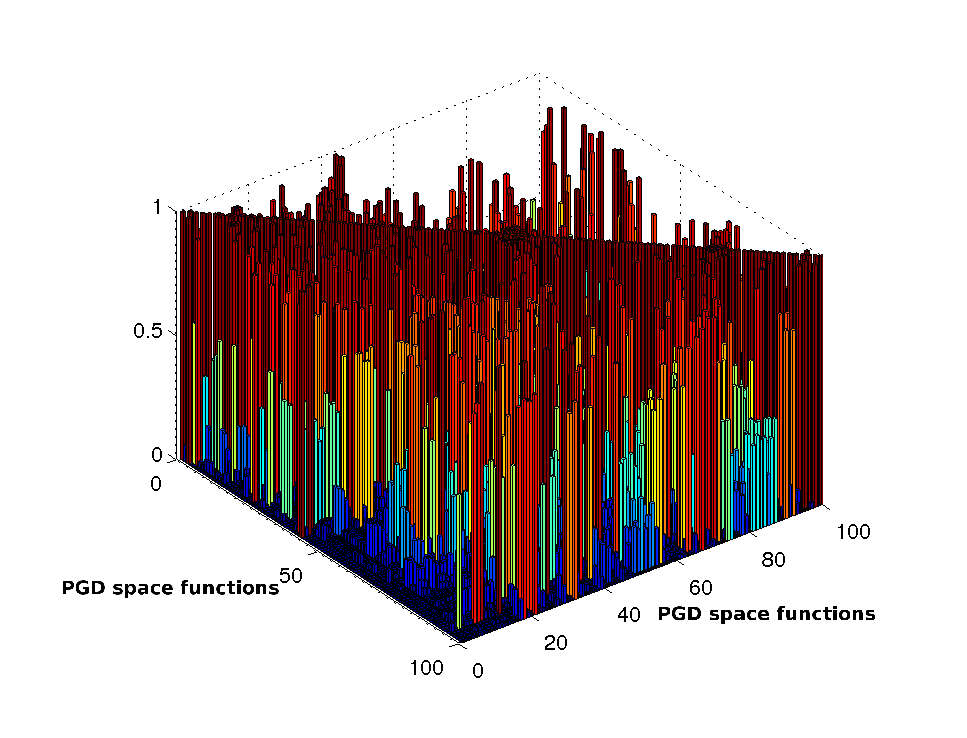
\includegraphics[width=1\linewidth]{MAC-PGD2.eps}
			\caption{\centering PGD space functions}		
		\end{minipage}
	\end{figure}
	\vspace{-0.75cm}
	\begin{itemize}
		\item POD : Orthogonality
			\vspace{-0.2cm}
		\item PGD : Correlation between mods
	\end{itemize}
\end{frame}

\begin{frame}{MAC Analysis
	$\frac{\left(\boldsymbol{\varphi_i.\psi_j}\right)^2}{\boldsymbol{\varphi_i.\varphi_i \times \psi_j.\psi_j}}$} 
	\vspace{-0.75cm}
	\begin{figure}
	%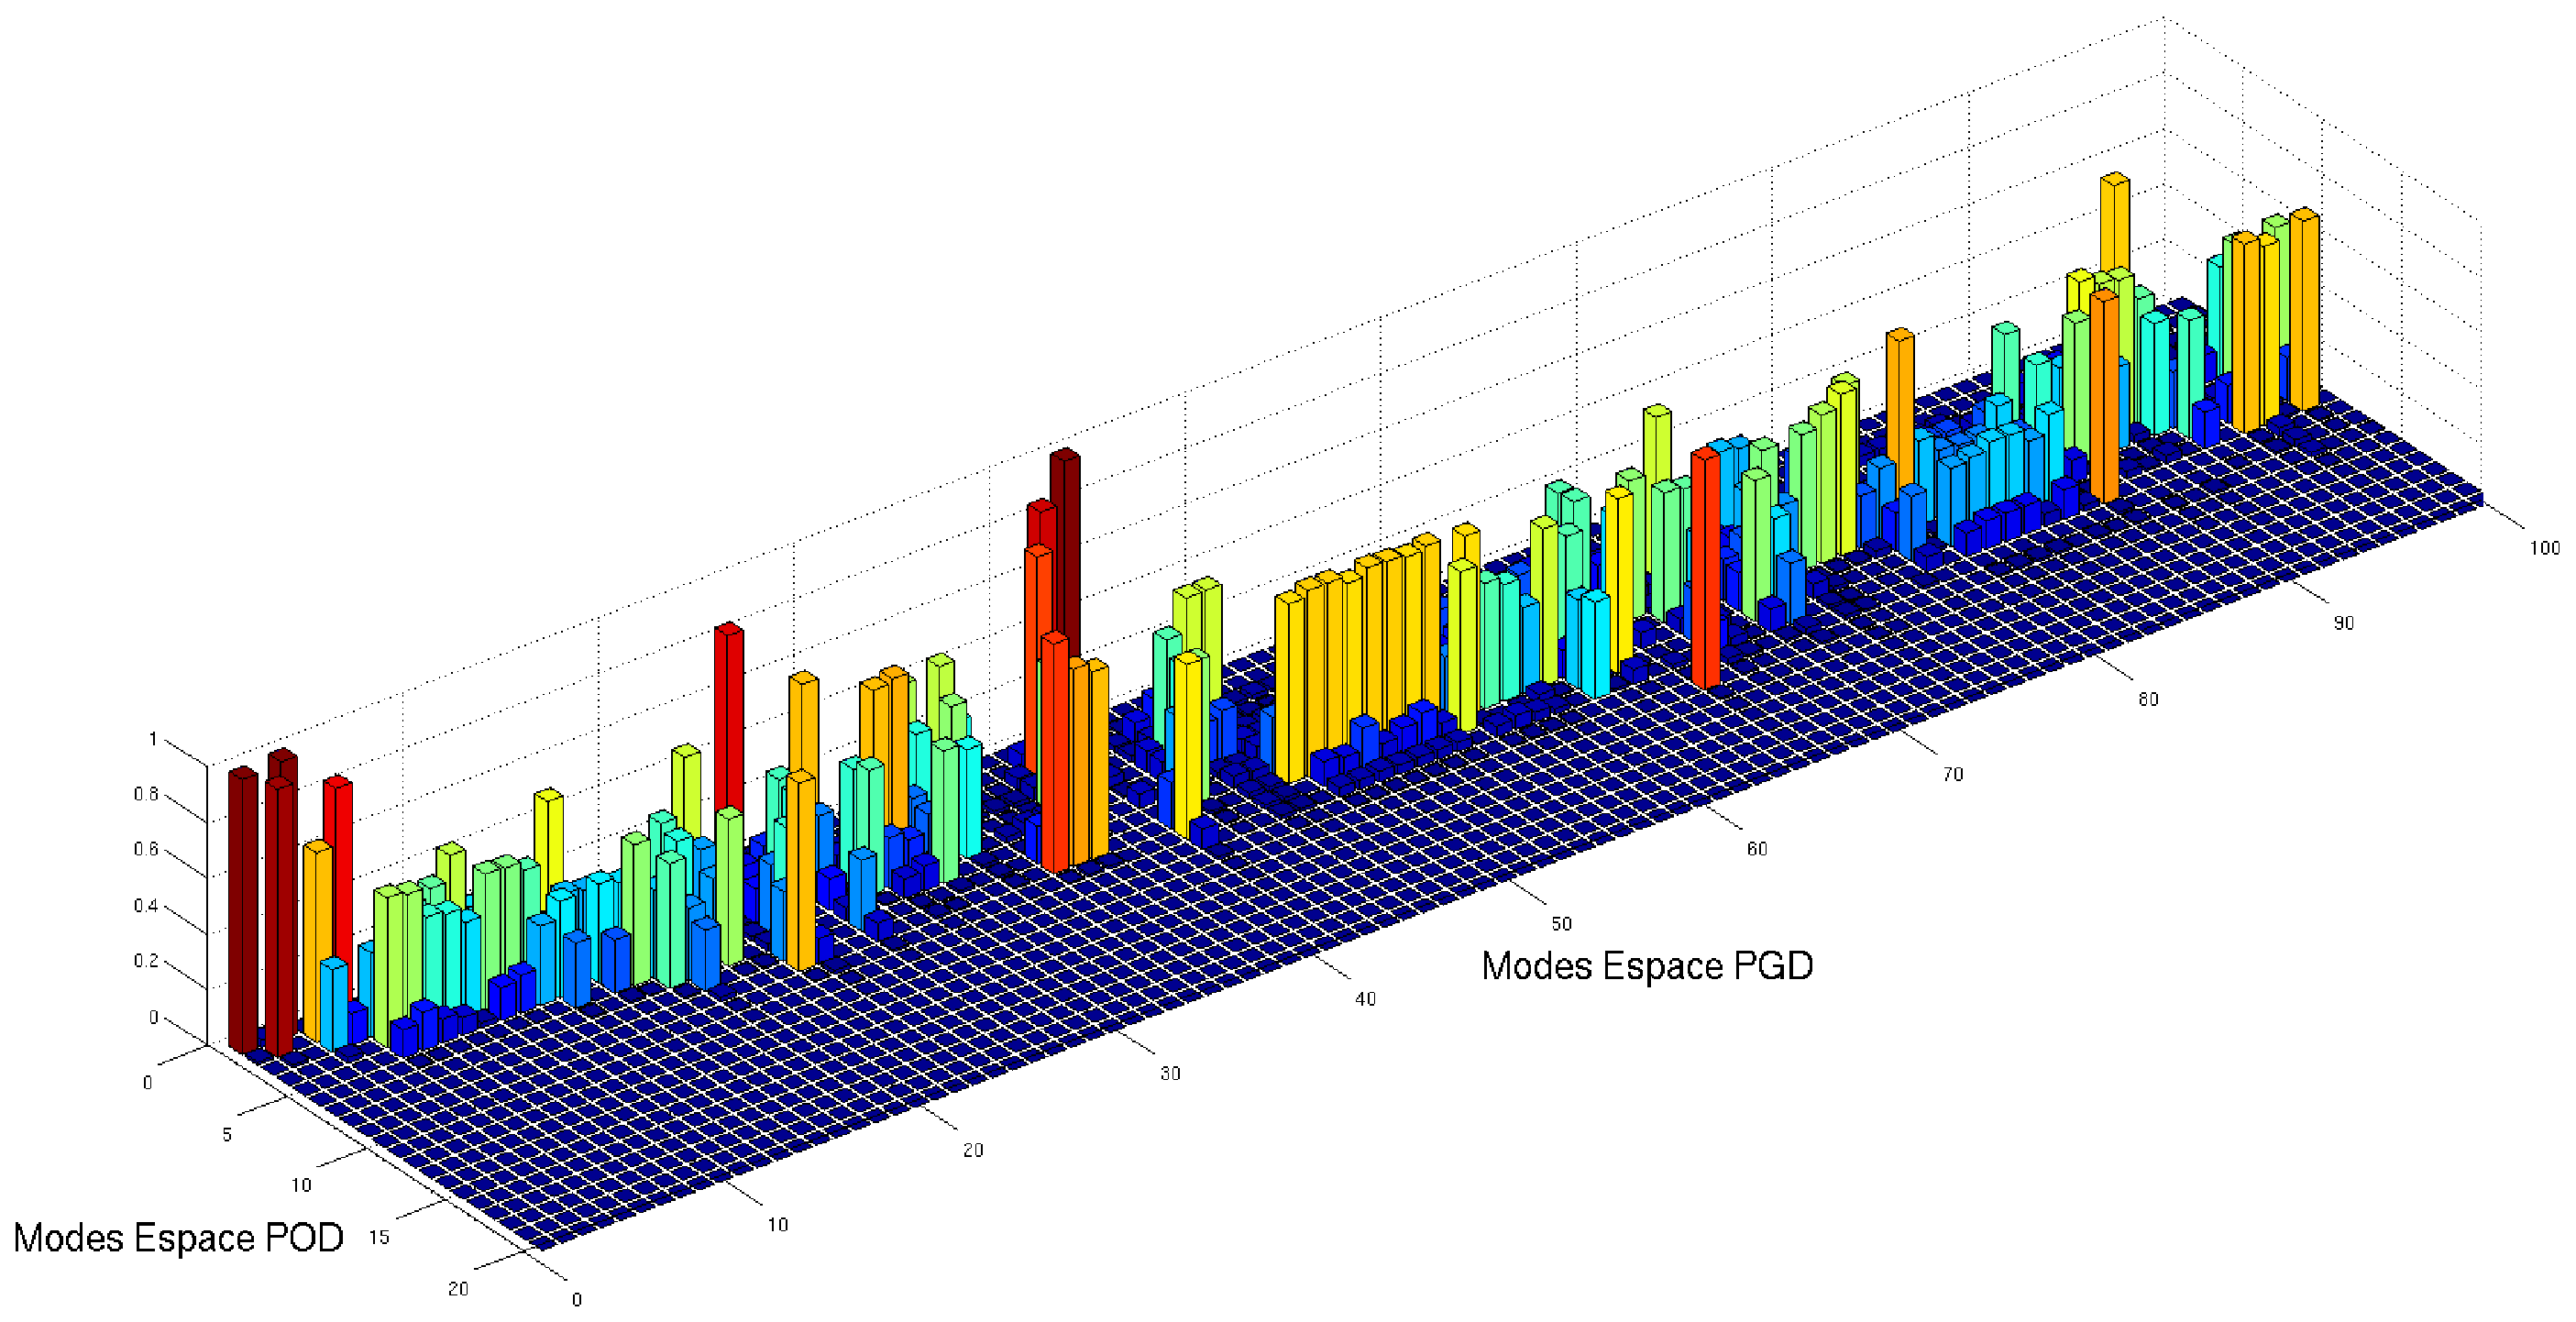
\includegraphics[width=0.9\linewidth]{100ModesAvecNormNonAmortiMAC.eps}
	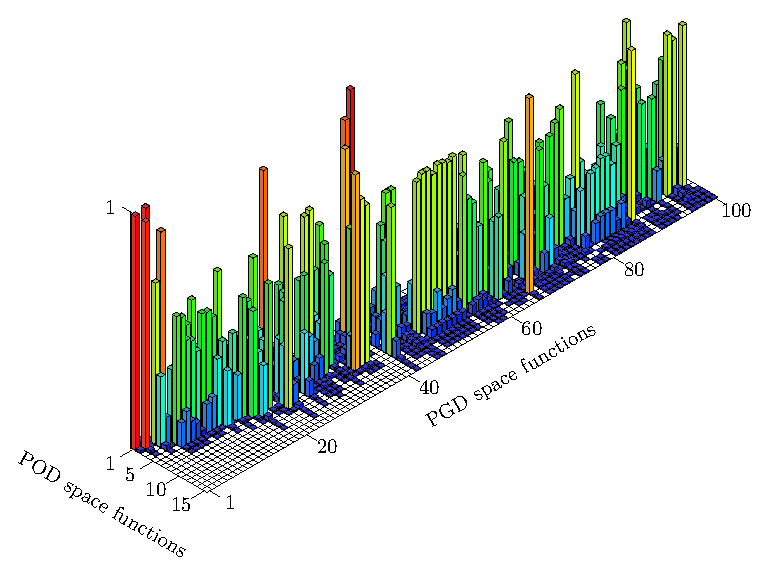
\includegraphics[width=0.7\linewidth]{MAC-POD-PGD.eps}
	\vspace{-0.4cm}
	\caption{Comparison between POD and PGD space functions}
	\end{figure}
	\vspace{-0.75cm}
	\begin{itemize}
		\item PGD mods only representing the first POD mods
	\end{itemize}
\end{frame}

\begin{frame}{Orthogonalization - 2 variables}
\FontPOD
\begin{figure}[t]
	$~$
	   \begin{minipage}[l]{0.43\linewidth}
			\begin{exampleblock}{Algorithm}
			\vbox to .4\textheight{%
				\vspace{0.42cm}
				$ ~~for~k = 1$ à $ n$ \\
				$ ~~\phantom{for} for~j=1$ à $j_{max}$ \\
				$ ~~\phantom{for for~j } f_k = F (U_{k-1},g_k)$ \\
				$ ~~\phantom{for for~j } g_k = G (U_{k-1},f_k)$ \\
				$ ~~\phantom{for} end$ \\
				$ ~~\phantom{for}\textcolor{red}{[f_k,g_{1..k-1}]=otho(f_{1..k},g_k)}$ \\
				$ ~~end $ \\				
			}
			\end{exampleblock}
	   \end{minipage}\hspace{0.05cm}
	   \begin{minipage}{0.49\linewidth}
			\begin{exampleblock}{Details \phantom{g}}
			\vbox to .4\textheight{%
				\[
				\begin{array}{l}
				~\text{Iterating on the modes }\\
				~ \phantom{for}\text{Using a fixed point loop}\\
				\phantom{for for}
				~\left\{
				\begin{array}{l l}
				&\!\!\!\!\!\!\!\!f_k = F (U_{k-1},g_k) \\
				&\!\!\!\!\!\!\!\!g_k = G (U_{k-1},f_k) \\			
				\end{array}
				\right.			\\
				~ \phantom{for} \text{to solve the non-linear problem.} \\
				~ \phantom{for} \textcolor{red}{Orthogonalizing}\\
				~\text{until you reach }n\text{ modes.}\\			
				\end{array}
				\]
			}
			\end{exampleblock}
	   \end{minipage}
	   
	\vspace{-0.6cm}
	\end{figure}
	\centering
	   \begin{minipage}{1\linewidth}
			\begin{exampleblock}{Gram-Schmidt}
				\vspace{-0.4cm}
				\[
				\begin{array}{l l l}
				U_k =	& \sum_{i=1}^{(k-1)}  f_i g_i &+ f_k g_k\\
							& + \sum_{i=1}^{(k-1)}  (f_i.f_k) f_i g_k &- \sum_{i=1}^{(k-1)}  (f_i.f_k) f_i g_k\\
				U_k = & \sum_{i=1}^{(k-1)} f_i \textcolor{blue}{(g_i+g_k(f_i.f_k))} &+ \textcolor{red}{(f_k-\sum_{i=1}^{(k-1)}(f_i.f_k)f_i )}g_k\\
				U_k =	& \sum_{i=1}^{(k-1)}  f_i \textcolor{blue}{g_i} &+ \textcolor{red}{f_k} g_k\\
				\end{array}
				\]
				\vspace{-0.3cm}
			\end{exampleblock}
	   \end{minipage}
\end{frame}


\begin{frame}{Orthogonalization - 3 variables}
\FontPOD

	\centering
	   \begin{minipage}{1\linewidth}
			\begin{exampleblock}{Gram-Schmidt}
				\vspace{-0.6cm}
				\[
				\begin{array}{l l l}
				U_k =	& \sum_{i=1}^{(k-1)}  f_i g_i h_i &+ f_k g_k h_k\\
							& + \sum_{i=1}^{(k-1)}  (f_i.f_k) f_i g_k h_k &- \sum_{i=1}^{(k-1)}  (f_i.f_k) f_i g_k h_k\\
				U_k = & \sum_{i=1}^{(k-1)} f_i \textcolor{blue}{(g_i h_i+g_k h_k(f_i.f_k))} 
								&+ \textcolor{red}{(f_k-\sum_{i=1}^{(k-1)}(f_i.f_k)f_i )}g_k h_k\\
				\end{array}
				\]
				% U_k =	& \sum_{i=1}^{(k-1)}  f_i \textcolor{blue}{g_i} &+ \textcolor{red}{f_k} g_k\\
				\vspace{-0.3cm}
			\end{exampleblock}
	   \end{minipage}
	   
	\centering
	   \begin{minipage}{0.9\linewidth}
			\begin{exampleblock}{Possibilities}
				\begin{itemize}
				 	\item Finding missing functions thanks to a minimization problem
				 	\item Orthogonalization afterwards or use the HOSVD
				\end{itemize}
			\end{exampleblock}
	   \end{minipage}
\end{frame}


	\begin{frame}
		\frametitle{Post processing of PGD modes}
		\framesubtitle{3 methods - MAC Analysis}
		\only<1>{
			\begin{figure}
				
\includegraphics[width=0.5\linewidth ,keepaspectratio]{Beam-tikz-0.eps}				
				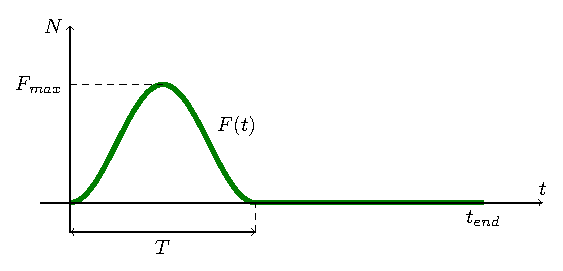
\includegraphics[width=0.5\linewidth ,keepaspectratio]{SinVerse-tikz.eps}	
			\end{figure}
		}
		\only<2>{
			\centering  SVD(PGD) - POD
			\\
			\vspace{0.5cm}
			\hspace{-1.2cm}
			\raisebox{-0.5\height}{	
				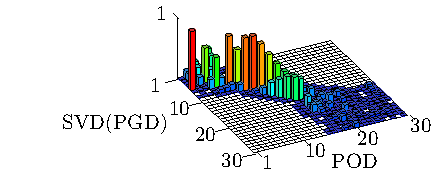
\includegraphics[trim=1cm 0cm 0cm 0cm, clip=true,width=0.55\linewidth ,keepaspectratio]{MacSVD(PGD)-POD.pdf}
				}
			\hspace{-0.7cm}
			\raisebox{-0.5\height}{	
				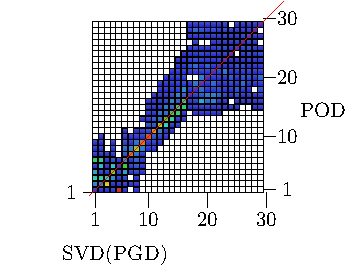
\includegraphics[trim=0.5cm 0cm 0cm 0cm, clip=true,width=0.55\linewidth ,keepaspectratio]{MacSVD(PGD)-POD-2.pdf}
				}
			\hspace{-1.5cm}
		}
		\only<3>{
			\centering  SVD(PGD Solution) - POD
			\\
			\vspace{0.5cm}
			\hspace{-1.2cm}
			\raisebox{-0.5\height}{	
				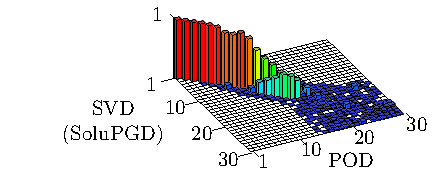
\includegraphics[trim=1cm 0cm 0cm 0cm, clip=true,width=0.55\linewidth ,keepaspectratio]{MacSVD(SoluPGD)-POD.pdf}
				}
			\hspace{-0.7cm}
			\raisebox{-0.5\height}{	
				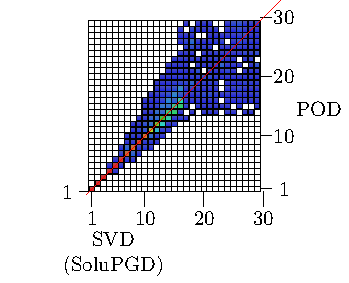
\includegraphics[trim=0.5cm 0cm 0cm 0cm, clip=true,width=0.55\linewidth ,keepaspectratio]{MacSVD(SoluPGD)-POD-2.pdf}
				}
			\hspace{-1.5cm}
		}
		\only<4>{
			\centering  SVD(weighted PGD) - POD
			\\
			\vspace{0.5cm}
			\hspace{-1.2cm}
			\raisebox{-0.5\height}{	
				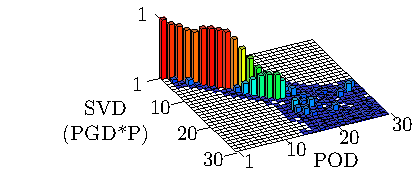
\includegraphics[trim=1cm 0cm 0cm 0cm, clip=true,width=0.55\linewidth ,keepaspectratio]{MacSVD(PGD-Ponderee)-POD.pdf}
				}
			\hspace{-0.7cm}
			\raisebox{-0.5\height}{	
				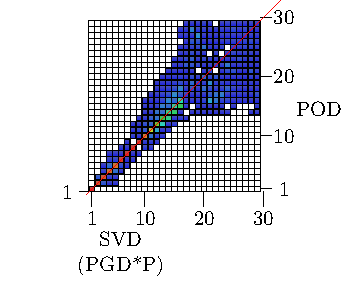
\includegraphics[trim=0.5cm 0cm 0cm 0cm, clip=true,width=0.55\linewidth ,keepaspectratio]{MacSVD(PGD-Ponderee)-POD-2.pdf}
				}
			\hspace{-1.5cm}
		}
		\only<5>{
			\centering  Singular values
			\\
			\raisebox{-0.5\height}{	
				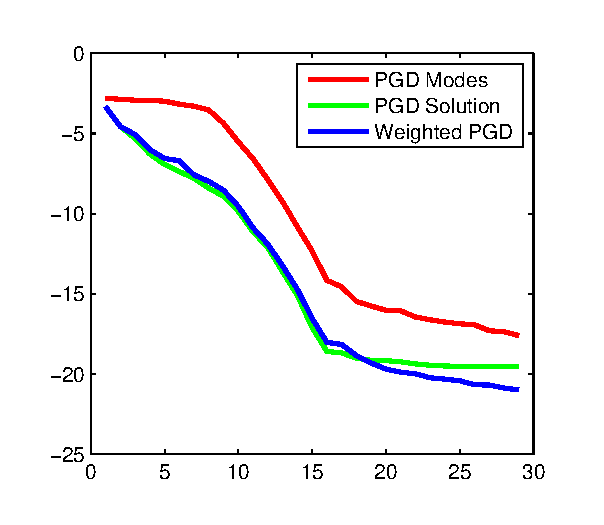
\includegraphics[trim=0cm 0.5cm 0cm 0.5cm, clip=true,width=1\linewidth, height=4.5cm ,keepaspectratio]{matValeursSinguliereTroisTests3.eps}
				}
				\begin{itemize}
					\item Lack of meaning from the SVD of the set of PGD modes
					\item Closes results for SVD of solution and SVD of weighted set
					\item $< 15$  meaningful modes
				\end{itemize}
		}
	
	\end{frame}
	
\section{Prospects}

\begin{frame}{Prospects}
\FontPersp
	\begin{itemize}
	
		\only<1-6>{
			\item Prepare program for Mecasif project test cases.
		}
		\only<1>{
				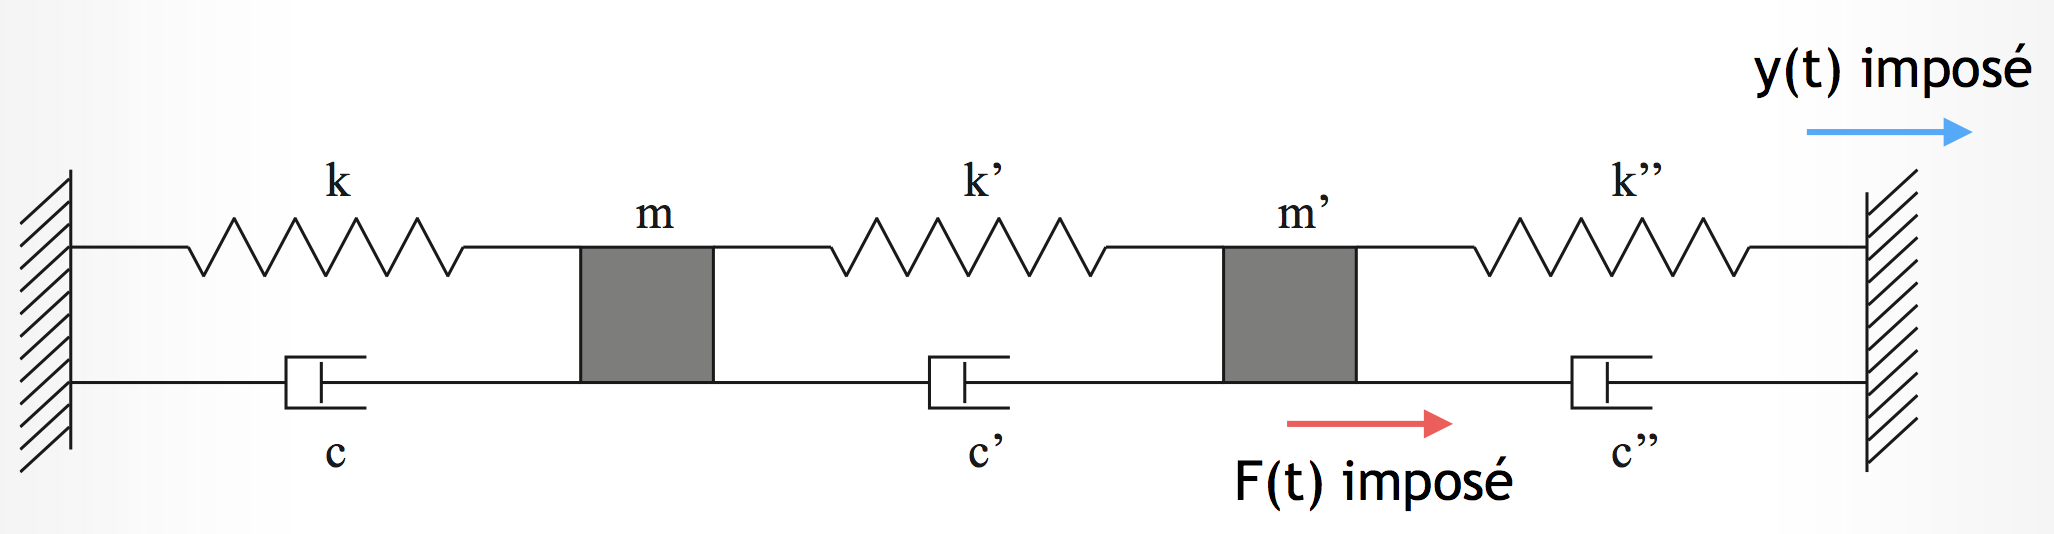
\includegraphics[trim=0cm 0cm 0cm 0cm, clip=true,width=\linewidth ,keepaspectratio]{CasTest1.png}
		}
		\only<2>{
				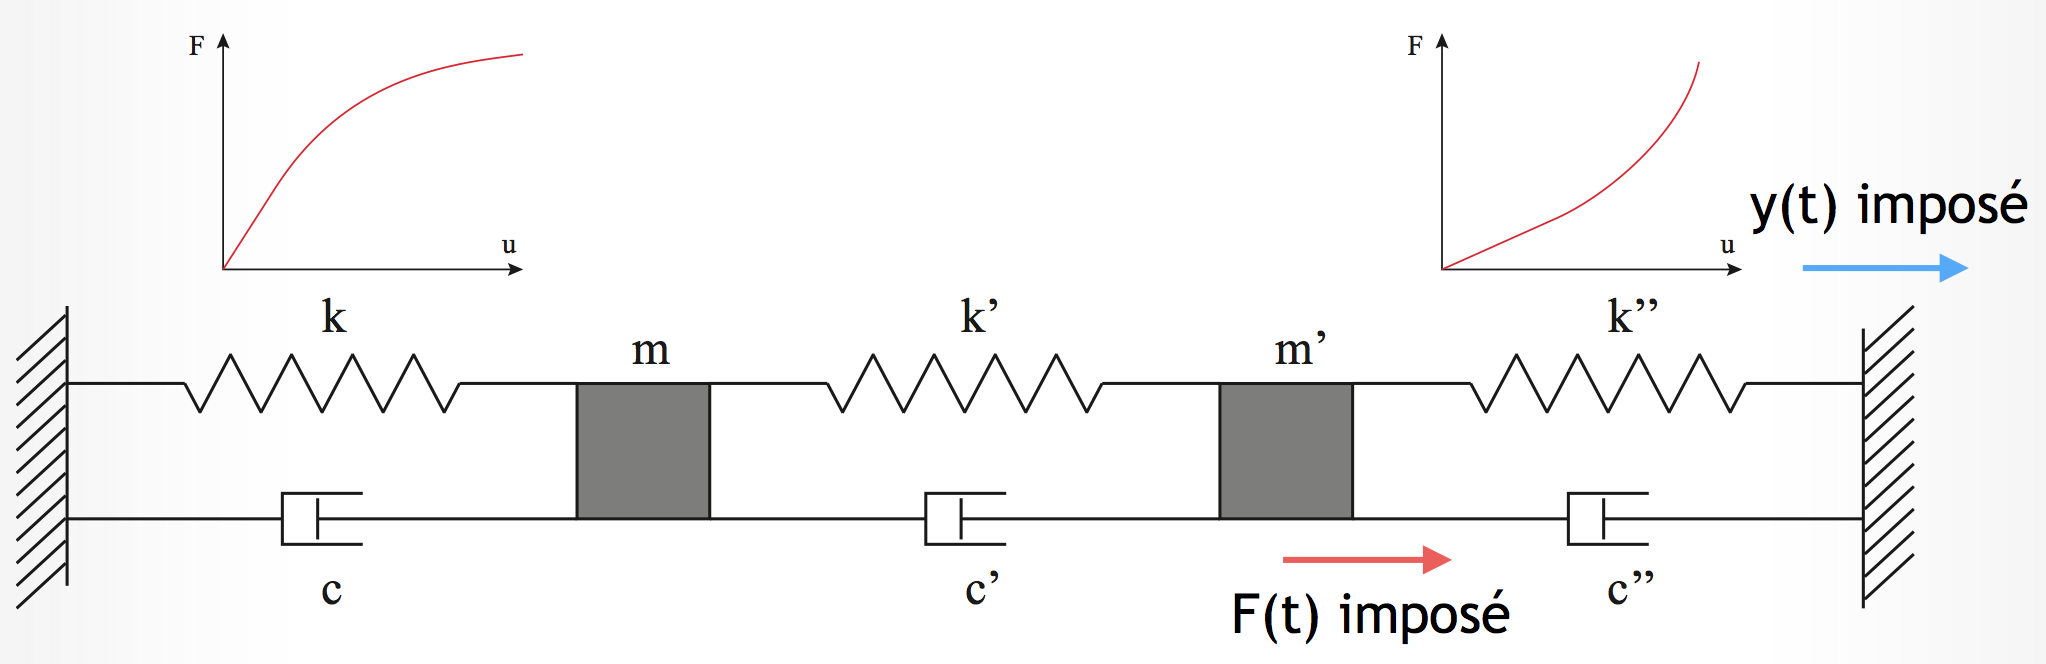
\includegraphics[width=\linewidth ,keepaspectratio]{CasTest2.png}
		}
		\only<3>{
				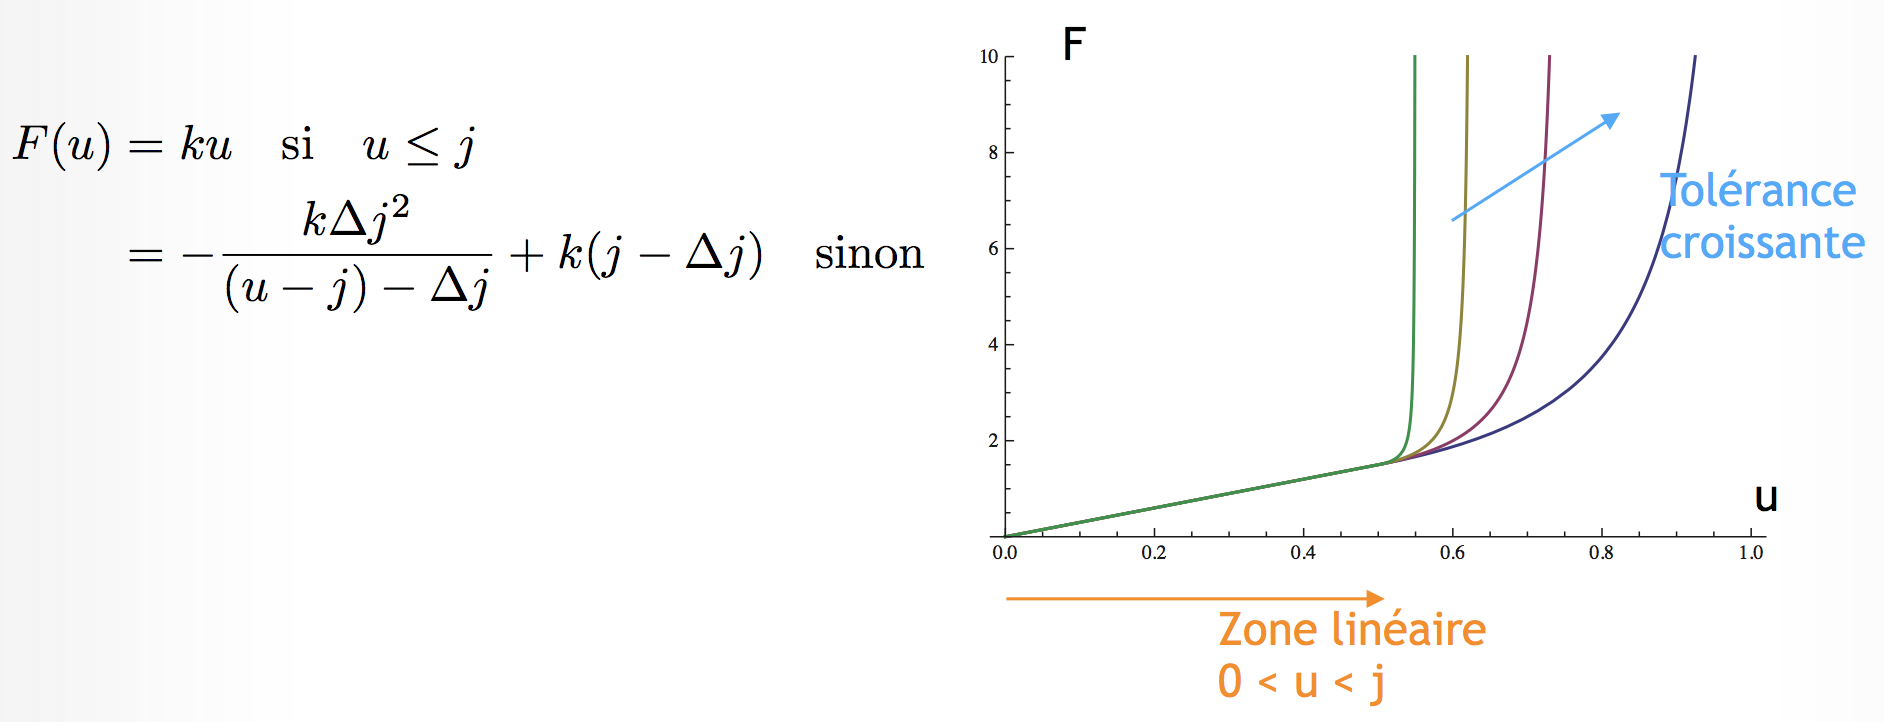
\includegraphics[width=\linewidth ,keepaspectratio]{FonctionButee.png}
		}
		\only<4>{
				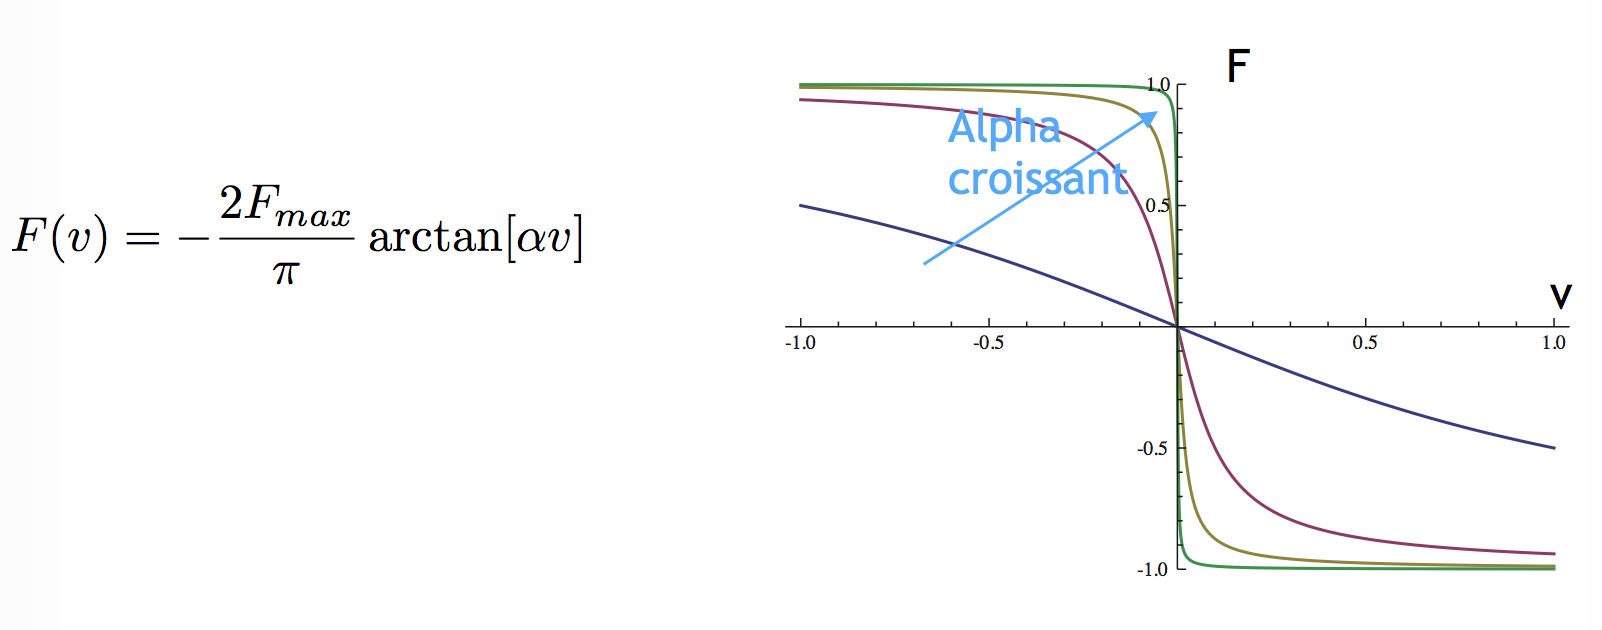
\includegraphics[width=\linewidth ,keepaspectratio]{FonctionContactFrottant.png}
		}
		\only<5>{
				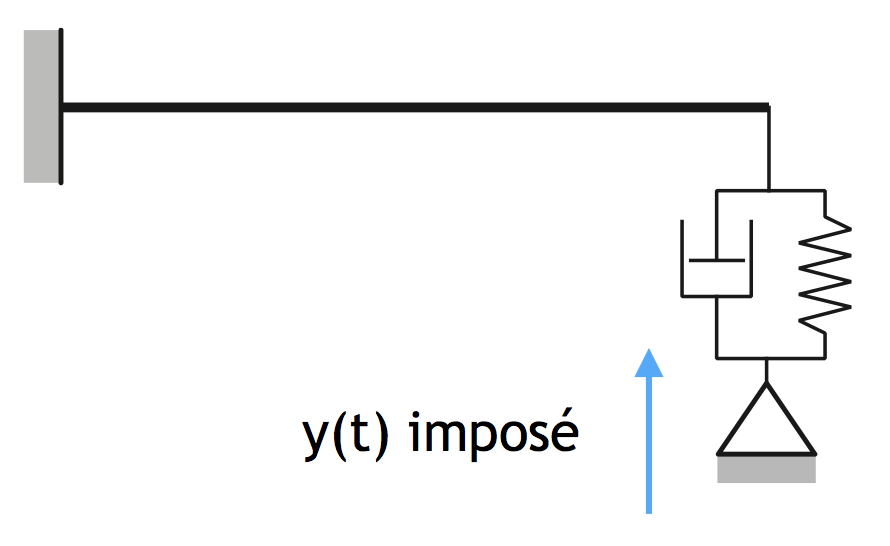
\includegraphics[width=0.7\linewidth ,keepaspectratio]{CasTest3.png}
		}
		\only<6>{
				\includegraphics[width=\linewidth ,keepaspectratio]{CasTest4.png}
		}
		\only<7>{
		\item Integration Scheme
			\begin{itemize}
			\FontPersp
			%\item Use of the Galerkin discontinous in time method for the PGD
			\item Influence of scheme dumping compared to problem dumping on PGD Convergence
			\end{itemize}
		\item Use SVD within the resolution to "clean" the PGD basis
		\item Integration in an open FE software
			%\begin{itemize}
			%\item SVD calculation implemented.
			%\end{itemize}
%		\item Add features present in other coworkers codes
%			\begin{itemize}
%			\FontPersp
%			\item Adding of parameter variables to the PGD %(Theorical calculation done.)
%			\end{itemize}
		\item Solving non-linear problems
			\begin{itemize}
			\FontPersp
			\item Use the test cases non-linearities
			\item Allow PGD non-linearities 
			\end{itemize}
		}
	\end{itemize}
\end{frame}



\end{document}
